\documentclass{article}
\usepackage[utf8]{inputenc}
\usepackage{tikz}
\usepackage{graphicx} % Required for inserting images
\usepackage{amsmath}
\usepackage{pgfplots}
\usetikzlibrary{patterns}
\usetikzlibrary{angles,quotes}
\usepackage{ amssymb }

\title{Kinematics}
\author{}
\date{}

\begin{document}

\maketitle

\section{Introduction}
Kinematics is the science of motion that treats the subject without regard to the forces that cause it. Within the science of kinematics, one studies the position, the velocity, the acceleration, and all higher order derivatives of the position variables(with respect to time or any other variable(s)).\\\\
Links and joints are the fundamental components of a robot. \textbf{Joints} represent movement on one rotational axis(x, y or z as rotational axis), or a one parameter translation(motion on x,y, or z axis)(one degree of freedom per joint). To fully represent an object in 3d space, we need six parameters; three for rotation $(\alpha,\beta,\gamma)$ and three for translation($(x,y,z)$-position of joint) (any more is considered redundant), because of this most robots are constructed using six joints to be able to fully express their position and orientation in 3d. \textbf{Links} are the static(unchanging) parts of a robot that connect joints to each other. Given n joints you will have n-1 links; think of links as edges and joints as nodes in a graph.\newpage
\textbf{Examples of joints:}\\
prismatic, spherical, planar(translation with one degree of freedom)\\
revolute, screw, cylindrical(rotational with one degree of freedom)\\
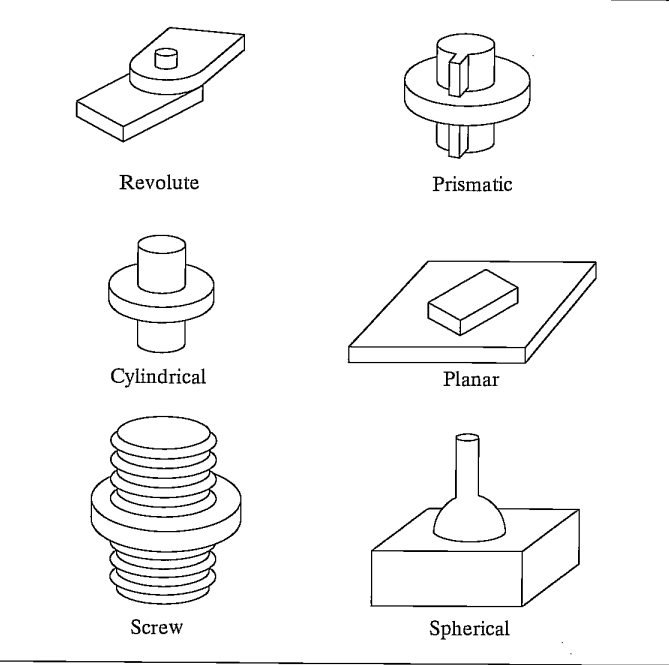
\includegraphics[width=7cm]{type_of_joints.png} \newpage

\section{Conventions for link-frame assignment}
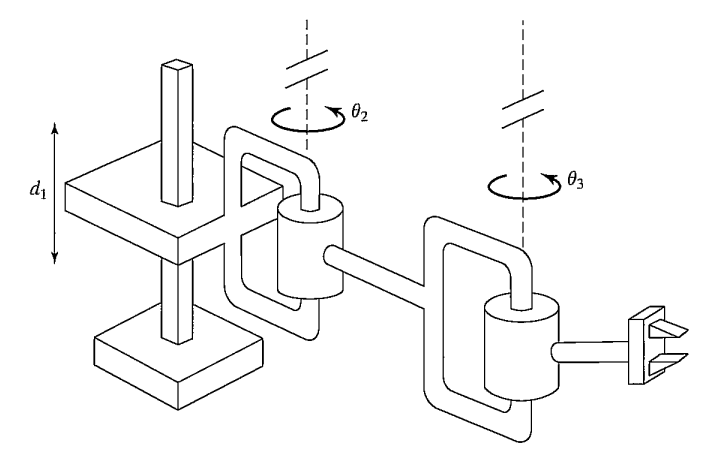
\includegraphics[width=7cm]{PRR.png}\\
\textbf{Algorithm: }\\
\textbf{1.} Identify the joint axes and imagine (or draw) infinite lines along them. For
steps 2 through 5 below, consider two of these neighboring lines (at axes i and
i + 1).\\\\
\textbf{2.} Identify the common perpendicular between them, or point of intersection.
At the point of intersection, or at the point where the common perpendicular
meets the ith axis, assign the link-frame origin.\\
\textbf{3.} Assign the $z_i$ axis pointing along the ith joint axis.\\
\textbf{4.}Assign the $x_i$ axis pointing along the common perpendicular, or, if the axes
intersect, assign $x_i$ to be normal to the plane containing the two axes.\\\\
\textbf{5.} Assign the $y_i$ axis to complete a right-hand coordinate system(optional step).\\\\
\textbf{6.} Assign frame \{0\} to match frame \{1\} when the first joint variable is zero. For {N}, choose an
origin location and $x_n$ direction freely, but generally so as to cause as many
linkage parameters as possible to become zero.\\\\
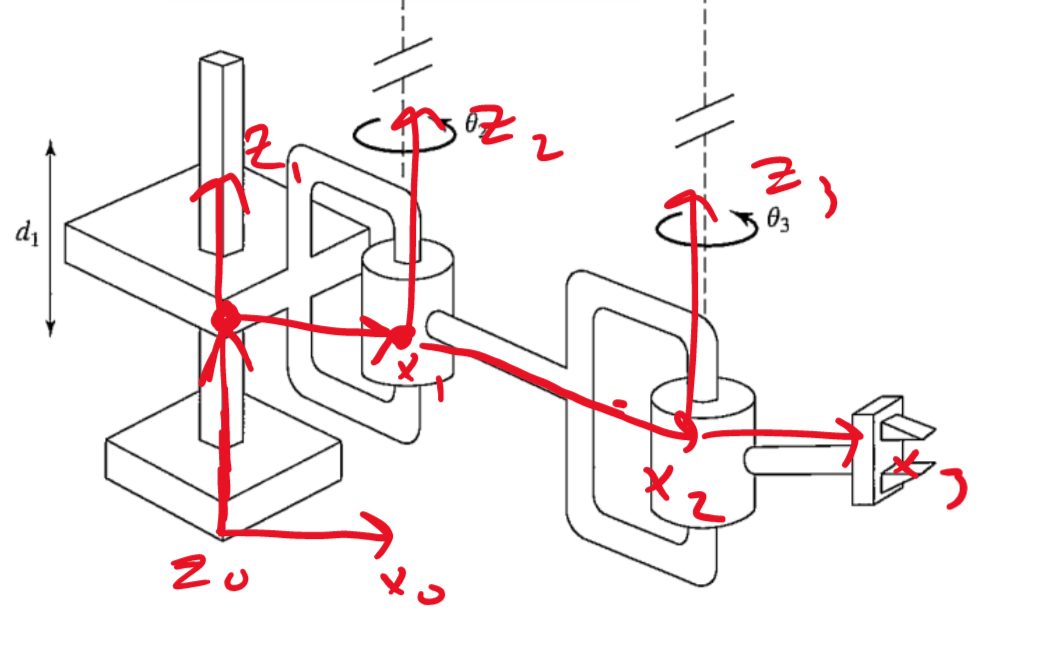
\includegraphics[width=7cm]{PRR_labeled.png}

\section{Parameters for dh table}
The DH table is a method for organizing parameters from a system of known joints, links, and frames. These parameters give us general formulas for constructing the transformations matrices required for computations. \\\\
$a_i$=Distance from $z_{i}$ to $z_{i+1}$ along the $x_i$(this is the link length, and mutual perpendicular between frame \{i\} and \{i+1\})\\\\
$\alpha_i$=link twist angle, angle from $z_{i}$ to $z_{i+1}$ measured along $x_{i}$ (angle between axis i and i+1)\\\\
$d_i$=link offset, the distance from $x_{i-1}$ to $x_{i}$ measured along $z_{i}$ (the offset distance of one link to the next)\\\\
$\theta_i$=the angle from $x_{i-1}$ to $x_{i}$ measured along $z_{i}$ (rotation of link w.r.t. its neighbor along common axis)\\\\

\begin{tabular}{ |p{3cm}|p{3cm}|p{3cm}| p{3cm} | p{3cm} |}
\hline
\multicolumn{5}{|c|}{DH table} \\
\hline
Frame \{i\} & \textbf{$a_{i-1}$} & \textbf{$\alpha_{i-1}$} & \textbf{$d_i$} & \textbf{$\theta_i$} \\
\hline
\textbf{1} & 0     & 0 & $d_1$ & $\theta_1=0$\\
\textbf{2} & $L_1$ & 0 & 0 & $\theta_2$\\
\textbf{3} & $L_2$ & 0 & 0 & $\theta_3$\\
\hline
\end{tabular}\\
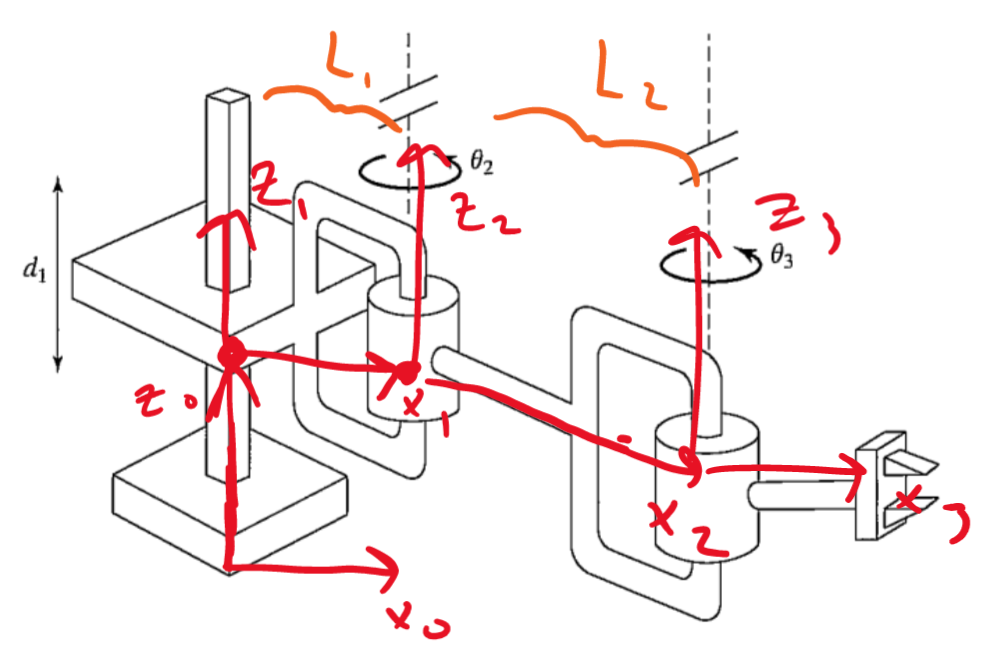
\includegraphics[width=7cm]{PRR_labeled2.png}

\section{dh table to transformation matrix}
Now that we have filled out the DH table, we can make all our transformation matrices using the matrix formula, Note the transformation uses rotation basis: $(R_z(\theta_i)R_x(\alpha_{i-1}))^T$. Tip - Each row corresponds to one transformation matrix, so row 1 has all the variables need for ${}^0_1T$, row 2 has all the variables for ${}^1_2T$ and so on.\\\\
${}^{i-1}_{i}T=\begin{bmatrix}
c\theta_i & -s\theta_i & 0 & a_{i-1}\\
s\theta_ic\alpha_{i-1} & c\theta_ic\alpha_{i-1} & -s\alpha_{i-1} & -s\alpha_{i-1}d_{i}\\
s\theta_is\alpha_{i-1} & c\theta_is\alpha_{i-1} & c\alpha_{i-1} & c\alpha_{i-1}d_{i}\\
                0 & 0 & 0 & 1
\end{bmatrix}$\\\\
\textbf{Note: } Use c0=1 and s0=0 to simplify.\\
${}^{0}_{1}T=
\begin{bmatrix}
c0 & -s0 & 0 & a_0\\
s0c0 & c0c0 & -s0 & -s0d_1\\
s0c0 & s0c0 & c0 & c0d_1\\
0 & 0 & 0 & 1
\end{bmatrix}=
\begin{bmatrix}
1 & 0 & 0 & 0\\
0 & 1 & 0 & 0\\
0 & 0 & 1 & d_1\\
0 & 0 & 0 & 1
\end{bmatrix}$\\\\
${}^{1}_{2}T=
\begin{bmatrix}
c\theta_2 & -s\theta_2 & 0 & L_1\\
s\theta_2c0 & c\theta_2c0 & -s0 & -s0d_2\\
s0c0 & s0c0 & c0 & c0d_2\\
0 & 0 & 0 & 1
\end{bmatrix}=
\begin{bmatrix}
c\theta_2 & -s\theta_2 & 0 & L_1\\
s\theta_2 & c\theta_2 & 0 & 0\\
0 & 0 & 1 & 0\\
0 & 0 & 0 & 1
\end{bmatrix}$\\\\
${}^{2}_{3}T=
\begin{bmatrix}
c\theta_3 & -s\theta_3 & 0 & L_2\\
s\theta_3c0 & c\theta_3c0 & -s0 & -s0d_3\\
s0c0 & s0c0 & c0 & c0d_3\\
0 & 0 & 0 & 1
\end{bmatrix}=
\begin{bmatrix}
c\theta_3 & -s\theta_3 & 0 & L_2\\
s\theta_3 & c\theta_3 & 0 & 0\\
0 & 0 & 1 & 0\\
0 & 0 & 0 & 1
\end{bmatrix}$\\\\
The whole system can be manipulated using the transformation:\\
${}^{0}_{3}T={}^{0}_{1}T{}^{1}_{2}T{}^{2}_{3}T = 
{}^0_3T =
\begin{bmatrix}
\cos(\theta_2+\theta_3) & -\sin(\theta_2+\theta_3) & 0 &
L_1 + L_2\cos\theta_2
\\[4pt]
\sin(\theta_2+\theta_3) & \cos(\theta_2+\theta_3) & 0 &
L_2\sin\theta_2
\\[4pt]
0 & 0 & 1 & d_1
\\[4pt]
0 & 0 & 0 & 1
\end{bmatrix}
$ \newpage

\section{2nd Example}
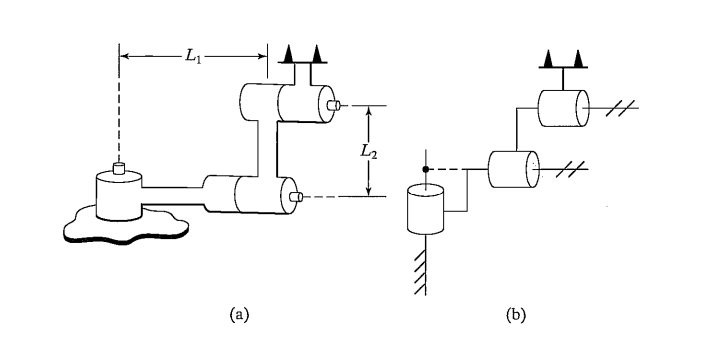
\includegraphics[width=10cm]{RRR_perp.png}\\
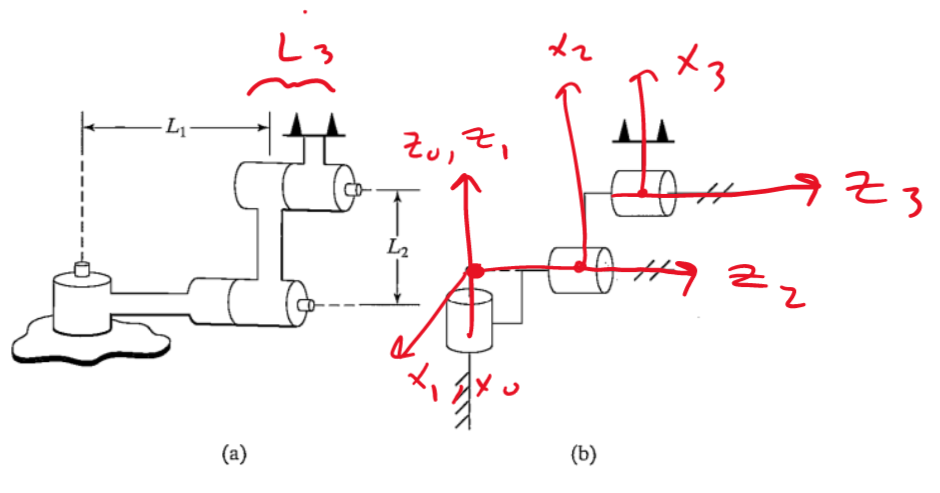
\includegraphics[width=10cm]{RRR_perp_labeled.png}\\\\
$a_0=dist(z_0,z_1) \text{ in } x_0=0\\
a_1=dist(z_1,z_2) \text{ in } x_1=0\\
a_2=dist(z_2,z_3) \text{ in } x_2=L_2\\\\
\alpha_0=angle(z_0,z_1) \text{ in } x_0=0\\
\alpha_1=angle(z_1,z_2) \text{ in } x_1=-90^\circ\\
\alpha_2=angle(z_2,z_3) \text{ in } x_2=0\\\\
d_1=dist(x_0,x_1) \text{ in } z_1=0\\
d_2=dist(x_1,x_2) \text{ in } z_2=L_1\\
d_3=dist(x_2,x_3) \text{ in } z_3=L_3\\\\
\theta_1=angle(x_0,x_1) \text{ in } z_1=\theta_1\\
\theta_2=angle(x_1,x_2) \text{ in } z_2=\theta_2-90^\circ\\
\theta_3=angle(x_2,x_3) \text{ in } z_3=\theta_3$\\\\
\begin{tabular}{ |p{3cm}|p{3cm}|p{3cm}| p{3cm} | p{3cm} |}
\hline
\multicolumn{5}{|c|}{DH table} \\
\hline
Frame \{i\} & \textbf{$a_{i-1}$} & \textbf{$\alpha_{i-1}$} & \textbf{$d_i$} & \textbf{$\theta_i$} \\
\hline
\textbf{1} & 0     & 0 & 0 & $\theta_1$\\
\textbf{2} & 0 & $-90^\circ$ & $L_1$ & $\theta_2-90^\circ$\\
\textbf{3} & $L_2$ & 0 & $L_3$ & $\theta_3$\\
\hline
\end{tabular}\\\\
Using
${}^{i-1}_{i}T=\begin{bmatrix}
c\theta_i & -s\theta_i & 0 & a_{i-1}\\
s\theta_ic\alpha_{i-1} & c\theta_ic\alpha_{i-1} & -s\alpha_{i-1} & -s\alpha_{i-1}d_{i}\\
s\theta_is\alpha_{i-1} & c\theta_is\alpha_{i-1} & c\alpha_{i-1} & c\alpha_{i-1}d_{i}\\
                0 & 0 & 0 & 1
\end{bmatrix}$ we get:\\\\
${}^{0}_{1}T=
\begin{bmatrix}
c\theta_1 & -s\theta_1 & 0 & 0\\
s\theta_1 & c\theta_1 & 0 & 0\\
0 & 0 & 1 & 0\\
0 & 0 & 0 & 1
\end{bmatrix}$\\\\
${}^{1}_{2}T=
\begin{bmatrix}
c(\theta_2-90^\circ) & -s(\theta_2-90^\circ) & 0 & 0\\
0 & 0 & 1 & L_1\\
s(\theta_2-90^\circ) & c(\theta_2-90^\circ) & 0 & 0\\
0 & 0 & 0 & 1
\end{bmatrix}$\\\\
${}^{2}_{3}T=
\begin{bmatrix}
c\theta_3 & -s\theta_3 & 0 & L_2\\
s\theta_3 & c\theta_3 & 0 & 0\\
0 & 0 & 1 & L_3\\
0 & 0 & 0 & 1
\end{bmatrix}$\\\\

Ultimately we get: 
\[
{}^0_3T =
\begin{bmatrix}
c_1 s_{23} & c_1 c_{23} & -s_1 &
L_2 c_1 s_2 - (L_1 + L_3)s_1
\\[4pt]
s_1 s_{23} & s_1 c_{23} & c_1 &
L_2 s_1 s_2 + (L_1 + L_3)c_1
\\[4pt]
c_{23} & -s_{23} & 0 &
L_2 c_2
\\[4pt]
0 & 0 & 0 & 1
\end{bmatrix}
\]

where: 
\[
c_1 = \cos\theta_1,\qquad
s_1 = \sin\theta_1
\]

\[
c_2 = \cos\theta_2,\qquad
s_2 = \sin\theta_2
\]

\[
c_{23} = \cos(\theta_2+\theta_3),\qquad
s_{23} = \sin(\theta_2+\theta_3)
\]


\section{Jacobian Matrix and Singularities}
Definition of Jacobian - multidimensional matrix of derivatives(J$\rightarrow$ velocity differentiate from positions), Jacobians can relate the joint velocities to cartesian(end effector) velocites in a robot manipulator.  \\\\
Cartesian: v=$\begin{bmatrix}
   \dot{ P_x} \\
    \dot{P_y} \\
    \dot{P_z}
\end{bmatrix}$ = Joint:$\begin{bmatrix}
                          {}^0v\\
                          {}^0w
\end{bmatrix} = J * \begin{bmatrix}
\dot{\theta_1} \\
\dot{\theta_2}
\end{bmatrix}$\\
${}^0v$ is linear\\
${}^0w$ is angular\\\\
You always need the jacobian in the base frame ${}^0J$, when you dont have it; you can solve for it. Use formula:\\
${}^0J={}^0_xR * {}^xJ$\\\\
Singularities- is a point where the robot loses one or more degrees of freedom. Here, it is impossible to move the end effector (tool) in a particular direction, regardless of the joint rates. two types: \\
\begin{itemize}
    \item Workspace-bound singularities- fully stretched out , or tool folded back on itself. Tool is at boundary of workspace.
    \item Workspace interior singularities - 2 or more joint axes line up with each other.
    \item At singularities robots lose their degrees of freedom. if the det[J($\theta)$]=0 singularity exist, if det[J($\theta)$]$\neq$0 no singularities. Remember $\theta=\begin{bmatrix}
        \theta_1 \\
        \theta_2\\
        ...\\
        \theta_n
    \end{bmatrix}$
\end{itemize}



\section{Jacobian Matrix -(to get robot velocities)}
Jacobian involves finding velocities. Steps:
\begin{itemize}
    \item DH table $\rightarrow$ Transformation matrix
    \item Get ${}^0_eT={}^0_1T {}^1_2T ... {}^n_eT$ and extract translation column to get P=$\begin{bmatrix}
        P_x\\
        P_y\\
        P_z
    \end{bmatrix}$ (position of end effector relative to base frame)
    \item When we differentiate P, we get: $\begin{bmatrix}
        \dot{P_x}\\
        \dot{P_y}\\
        \dot{P_z}
    \end{bmatrix}= {}^0J \begin{bmatrix}
        \dot{\theta_1} \\
        \dot{\theta_2} \\
        \dot{\theta_3}
    \end{bmatrix}$
\end{itemize}
\textbf{General formula:}\\
Given position of joints:
\begin{itemize}
    \item $y_1=f_1(x_1,x_2,...)$
    \item $y_2=f_2(x_1,x_2,...)$
    \item ...
    \item $y_n=f_n(x_1,x_2,...)$
\end{itemize}
We can then differentiate to get:
\begin{itemize}
    \item $\partial y_1=f_1(\frac{\partial f_1}{\partial x_1}\partial x_1,\frac{\partial f_1}{\partial x_2}\partial x_2,...)$
    \item $\partial y_2=f_2(\frac{\partial f_2}{\partial x_1}\partial x_1,\frac{\partial f_2}{\partial x_2}\partial x_2,...)$
    \item ...
    \item $\partial y_n=f_n(\frac{\partial f_n}{\partial x_1}\partial x_1,\frac{\partial f_n}{\partial x_2}\partial x_2,...)$
\end{itemize}
In Matrix form:
$\dot{Y}=J\dot{X} \rightarrow \begin{bmatrix}
    \dot{y_1}\\
    \dot{y_2}\\
    ...
\end{bmatrix}=
\begin{bmatrix}
    \frac{\partial F}{\partial X} = J 
\end{bmatrix}\begin{bmatrix}
    \dot{x_1}\\
    \dot{x_2}\\
    ...
\end{bmatrix}$
\subsection{Example}
\textbf{Q:} Velocity of the tip of the arm as a function of joint rates

\begin{enumerate}
    \item[(i)] Give the answer in terms of frame 0
    \item[(ii)] Give the answer in terms of frame 2
\end{enumerate}

\vspace{1cm}

% Simple representation of the 2-link robot arm
\begin{center}
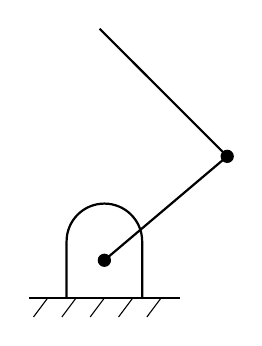
\begin{tikzpicture}[scale=1.2]

    % Ground
    \draw[thick] (-0.8,0) -- (0.8,0);
    \foreach \x in {-0.6,-0.3,0,0.3,0.6}
        \draw (\x,0) -- (\x-0.15,-0.2);

    % Base
    \draw[thick] (-0.4,0) -- (-0.4,0.6)
                 arc[start angle=180,end angle=0,radius=0.4]
                 -- (0.4,0);

    % Joint 1
    \fill (0,0.4) circle (2pt);

    % Link 1
    \draw[thick] (0,0.4) -- (1.3,1.5);

    % Joint 2
    \fill (1.3,1.5) circle (2pt);

    % Link 2
    \draw[thick] (1.3,1.5) -- (0.3,2.5);

    % End effector
    \draw[thick] (0.15,2.65) -- (0.45,2.35);
    \draw[thick] (0.15,2.65) -- (-0.05,2.85);

\end{tikzpicture}
\end{center}

\vspace{0.5cm}

\begin{center}
\renewcommand{\arraystretch}{1.5}
\begin{tabular}{|c|c|c|c|c|}
\hline
\textbf{Axis $(i)$} &
$\boldsymbol{\alpha_{i-1}}$ &
$\boldsymbol{a_{i-1}}$ &
$\boldsymbol{d_i}$ &
$\boldsymbol{\theta_i}$ \\ \hline

1 & $0$ & $L_1$ & $0$ & $\theta_1$ \\ \hline

2 & $0$ & $L_2$ & $0$ & $\theta_2$ \\ \hline

\end{tabular}
\end{center}



\textbf{Part 1} using kinematics formula to get:\\
${}^0_1T=\begin{bmatrix}
c\theta_1 & -s\theta_1 & 0 & l_1 \\
s\theta_1 & c\theta_1 & 0 & 0 \\
0 & 0 & 1 & 0 \\
0 & 0 & 0 & 1 \\
\end{bmatrix}$\\
${}^1_2T=\begin{bmatrix}
c\theta_2 & -s\theta_2 & 0 & l_2 \\
s\theta_2 & c\theta_2 & 0 & 0 \\
0 & 0 & 1 & 0 \\
0 & 0 & 0 & 1 \\
\end{bmatrix}$\\\\
Now we can solve for:\\
${}^0_2T=\begin{bmatrix}
c_{12} & -s{12} & 0 & l_1 + l_2 c\theta_1\\
s{12} & c{12} & 0 & l_2 s\theta_1 \\
0 & 0 & 1 & 0 \\
0 & 0 & 0 & 1 \\
\end{bmatrix}$\\
Giving us : $P=\begin{bmatrix}
              l_1 + l_2 c\theta_1\\
              l_2 s\theta_1\\
              0
\end{bmatrix}$ thus, :
$\dot{P}=\begin{bmatrix}
    -l_2s\theta_1 \dot{\theta_1}\\
    l_2c\theta_1 \dot{\theta_1}\\
    0
\end{bmatrix}$ We can then write: $\dot{P}=\begin{bmatrix}
    -l_2s\theta_1\\
    l_2c\theta_1\\
    0
\end{bmatrix}\begin{bmatrix}
    \dot{\theta_1}
\end{bmatrix}$ where this is equivalent to $\dot{Y}=J\dot{X}$ and ${}^0V={}^0J[\dot{\theta_1}]$\\
\textbf{ANSWERS QUESTION VELOCITY OF THE TOOL(FRAME 2) RELATIVE TO FRAME 0}\\\\
\textbf{Part 2}\\
Solve ${}^2V={}^2J[\dot{\theta_1}]$. Using formula:\\
${}^2J={}^2_0 R {}^0J$\\
From previous question, where we solved for ${}^0_2 T$ we can extract ${}^0_2 R$ and take transpose to get:\\
${}^2_0 R=\begin{bmatrix}
c_{12} & s{12} & 0 \\
-s{12} & c{12} & 0 \\
0 & 0 & 1\\
\end{bmatrix}$ so, we get:\\
${}^2J=\begin{bmatrix}
c_{12} & s{12} & 0 \\
-s{12} & c{12} & 0 \\
0 & 0 & 1\\
\end{bmatrix}
\begin{bmatrix}
-l_2s\theta_1\\
l_2c\theta_1\\
0
\end{bmatrix}=
\begin{bmatrix}
-l_2c_{12}s_1 + l_2s_{12}c_1\\
l_2s_{12}s_1 + l_2c_{12}c_1\\
0
\end{bmatrix}$\\ and finally solving for ${}^2v$, we get:\\
${}^2v=\begin{bmatrix}
-l_2c_{12}s_1 + l_2s_{12}c_1\\
l_2s_{12}s_1 + l_2c_{12}c_1\\
0
\end{bmatrix}\begin{bmatrix}
\dot{\theta_1}
\end{bmatrix}$\\\\

\section{Jacobian Matrix - Velocity Propagation Method}
\textbf{Intro Steps:} 
\begin{itemize}
    \item Get linear velocity (v)
    \item Get angular velocity ($\omega$)
    \item Start from first frame and solve eqns till you get to end effector frame $0 \rightarrow 1 \rightarrow 2 \rightarrow ... \rightarrow E$
    \item ${}^E V_E = {}^E J \begin{bmatrix}
         \dot{\theta_1} \\
        \dot{\theta_2} 
    \end{bmatrix}$\\\\
    ${}^0J={}^0_ER * {}^EJ$
\end{itemize}
\textbf{Linear Velocity}\\
Consider two frames \{A\},\{B\}; where \{A\} is fixed  and \{B\} is moving away from \{A\}. Orientation of \{B\} does not change. Let Frame \{B\} have a point Q(${}^BP_Q$). We can compute the linear velocity of ${}^BP_Q$ with respect to frame \{A\} using the formula: \\
${}^AV_Q = {}^AV_B + {}^A_BR {}^BV_Q$

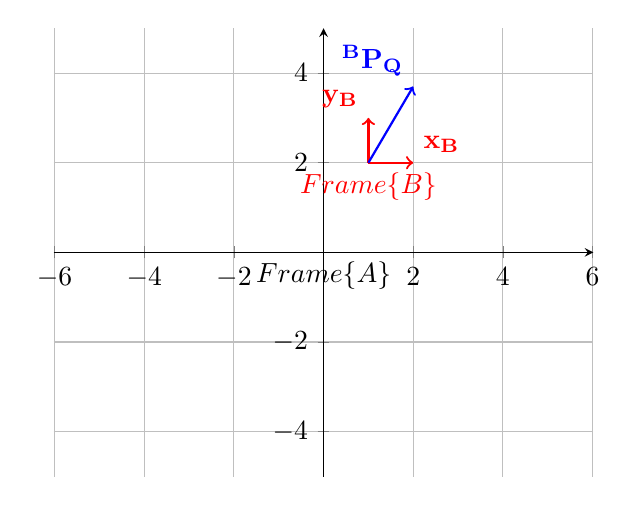
\begin{tikzpicture}
\begin{axis}[axis lines=middle, xmin=-5, xmax=5, ymin=-5,ymax=5,axis equal,grid=both]
\addplot [->, thick,  red] coordinates { (1,2) (2,2)}node[above right]{$\mathbf{x_B}$};
\addplot [->, thick,  red] coordinates { (1,2) (1,3)}node[above left]{$\mathbf{y_B}$};
\addplot [->, thick,  blue] coordinates { (1,2) (2,3.7)}node[above left]{$\mathbf{^BP_Q}$};
\addplot [red] coordinates { (1,2) (1,2)}node[below]{$Frame \{B\}$};
\addplot [black] coordinates { (0,0) (0,0)}node[below]{$Frame \{A\}$};
\end{axis}
\end{tikzpicture}\\\\\\
\textbf{Angular Velocity}\\
Consider two frames \{A\},\{B\}; where \{A\} is fixed  and \{B\} is moving away from \{A\}. No linear motion for \{B\}. Let Frame \{B\} have a point Q(${}^BP_Q$). We can compute the angular velocity of ${}^BP_Q$ with respect to frame \{A\} using the formula: \\
${}^AV_Q = {}^A_BR {}^BV_Q + {}^A_B\Omega \times {}^A_BR {}^BP_Q$

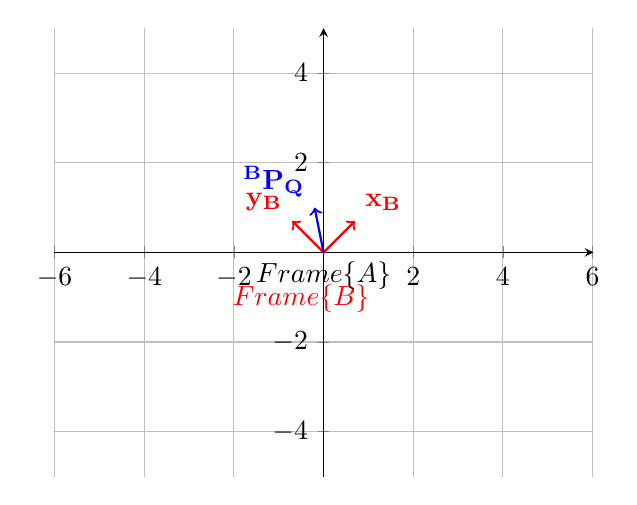
\begin{tikzpicture}
\begin{axis}[axis lines=middle, xmin=-5, xmax=5, ymin=-5,ymax=5,axis equal,grid=both]
\addplot [->, thick,  red] coordinates { (0,0) (.7,.7)}node[above right]{$\mathbf{x_B}$};
\addplot [->, thick,  red] coordinates { (0,0) (-.7,.7)}node[above left]{$\mathbf{y_B}$};
\addplot [->, thick,  blue] coordinates { (0,0) (-.2,1)}node[above left]{$\mathbf{^BP_Q}$};
\addplot [red] coordinates { (-.5,-.5) (-.5,-.5)}node[below]{$Frame \{B\}$};
\addplot [black] coordinates { (0,0) (0,0)}node[below]{$Frame \{A\}$};
\end{axis}
\end{tikzpicture}

\subsection{Velocity Propagation equations(iterative)}
1. ${}^{i+1}\omega_{i+1}={}^{i+1}_iR({}^i \omega_i) + \dot{\theta}_{i+1} {}^{i+1}\hat{z}_{i+1}$\\
2. ${}^{i+1}v_{i+1}={}^{i+1}_iR({}^i v_i + {}^i \omega_i \times {}^i P_{i+1}) + \dot{d}_{i+1} {}^{i+1}\hat{z}_{i+1}$\\\\
\begin{itemize}
    \item i is joint/frame
    \item i+1 next frame
    \item $\omega$ angular velocity
    \item $v$ linear velocity
    \item $\dot{\theta}_{i+1} \hat{z}$ is for revolute joints: $\begin{bmatrix}
        0\\
        0\\
        \dot{\theta}_{i+1}
    \end{bmatrix}$
    \item $\dot{d}_{i+1} \hat{z}$ is for prismatic joints: $\begin{bmatrix}
        0\\
        0\\
        \dot{d}_{i+1}
    \end{bmatrix}$
    \item The main idea is starting from frame \{0\} iteratively solve the solution for $n$ joints. 
\end{itemize}

\subsection{Example}
\begin{enumerate}
    \item[(a)] Find the \textbf{linear and angular velocity} at the last frame

    \item[(b)] Find the \textbf{Jacobian} at the last frame

    \item[(c)] Find the \textbf{Jacobian} at the base frame

    \item[(d)] Find an equation for the \textbf{singularities} of the robot
\end{enumerate}

\vspace{0.5cm}

\noindent
The solution procedure is:

\begin{enumerate}
    \item DH Table
    \item Transformation matrices
    \item Velocity propagation: base $\rightarrow$ final
    \item ${}^{3}J$
    \item ${}^{0}J$
    \item Singularities
\end{enumerate}

\vspace{1cm}

Define

\[
c_i = \cos\theta_i,
\qquad
s_i = \sin\theta_i.
\]

The individual transformation matrices are

\[
{}^{0}_{1}T =
\begin{bmatrix}
c_1 & -s_1 & 0 & 0 \\
s_1 &  c_1 & 0 & 0 \\
0   &  0   & 1 & 0 \\
0   &  0   & 0 & 1
\end{bmatrix},
\]

\[
{}^{1}_{2}T =
\begin{bmatrix}
-s_2 & -c_2 & 0  & 0 \\
0    & 0    & -1 & 0 \\
c_2  & -s_2 & 0  & 0 \\
0    & 0    & 0  & 1
\end{bmatrix},
\]

and

\[
{}^{2}_{3}T =
\begin{bmatrix}
1 & 0 & 0  & 0 \\
0 & 0 & -1 & -d_3 \\
0 & 1 & 0  & 0 \\
0 & 0 & 0  & 1
\end{bmatrix}.
\]

Multiplying the transformations gives

\[
{}^{0}_{3}T
=
{}^{0}_{1}T
{}^{1}_{2}T
{}^{2}_{3}T,
\]

so that

\[
\boxed{
{}^{0}_{3}T =
\begin{bmatrix}
-c_1s_2 & s_1 & c_1c_2 & c_1c_2d_3 \\
-s_1s_2 & c_1 & s_1c_2 & s_1c_2d_3 \\
c_2     & 0   & s_2     & s_2d_3 \\
0       & 0   & 0       & 1
\end{bmatrix}
}
\]


\subsection*{Robot Configuration}

\begin{center}
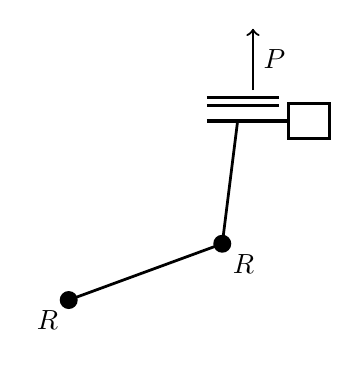
\begin{tikzpicture}[scale=1.3, line width=1pt]

% First revolute joint
\fill (0,0) circle (2.5pt);
\node[below left] at (0,0) {$R$};

% First link
\draw (0,0) -- (1.5,0.55);

% Second revolute joint
\fill (1.5,0.55) circle (2.5pt);
\node[below right] at (1.5,0.55) {$R$};

% Vertical link
\draw (1.5,0.55) -- (1.65,1.75);

% Prismatic joint / slider
\draw[line width=1.5pt] (1.35,1.75) -- (2.15,1.75);

% Slider block
\draw (2.15,1.58) rectangle (2.55,1.92);

% Prismatic direction
\draw[->, thick] (1.8,2.05) -- (1.8,2.65);
\node[right] at (1.8,2.35) {$P$};

% small parallel lines indicating prismatic joint
\draw (1.35,1.90) -- (2.05,1.90);
\draw (1.35,1.98) -- (2.05,1.98);

\end{tikzpicture}
\end{center}

Thus, the robot has the joint sequence

\[
\boxed{R-R-P}
\]

where the first two joints are revolute and the third joint is
prismatic.


\subsubsection{Part A(solution)}
Base frame usually never moves so we can say:\textbf{frame\{0\}}\\
${}^0\omega_0={}^0v_0=\begin{bmatrix}
0\\
0\\
0
\end{bmatrix}$\\\\
\textbf{Frame \{1\}} iteration(i=0):\\
1. ${}^1 \omega_1 = {}^1_0R ({}^0 \omega_0) + \dot{\theta}_1 \hat{z} = \begin{bmatrix}
    0\\
    0\\
    \dot{\theta}_1
\end{bmatrix}$\\
2. ${}^{1}v_{1}={}^{1}_0R({}^0 v_0 + {}^0 \omega_0 \times {}^0 P_{1}) + \dot{d}_{1} {}^{1}\hat{z}_{1}=\begin{bmatrix}
    0\\
    0\\
    0
\end{bmatrix}$ $\dot{d}_{1} {}^{1}\hat{z}_{1}$ goes to zero cause revolute joint here.\\\\
\textbf{Frame \{2\}} iteration(i=1):\\
1. ${}^2 \omega_2 = {}^2_1R ({}^1 \omega_1) + \dot{\theta}_2 \hat{z} =\begin{bmatrix}
-s_2 & 0 & c_2\\
-c_2 & 0 & -s_2\\
0 & -1 & 0
\end{bmatrix} \begin{bmatrix}
    0\\
    0\\
    \dot{\theta}_1
\end{bmatrix} + \begin{bmatrix}
0\\
0\\
\dot{\theta}_2
\end{bmatrix} = \begin{bmatrix}
    c_2\dot{\theta}_1\\
    -s_2\dot{\theta}_1\\
    \dot{\theta}_2
\end{bmatrix}$\\
2. ${}^{2}v_{2}={}^{2}_1R({}^1 v_1 + {}^1 \omega_1 \times {}^1 P_{2}) + \dot{d}_{2} {}^{2}\hat{z}_{2}=
\begin{bmatrix}
-s_2 & 0 & c_2\\
-c_2 & 0 & -s_2\\
0 & -1 & 0
\end{bmatrix} (\begin{bmatrix}
    0\\
    0\\
    0
\end{bmatrix} + \begin{bmatrix}
    0\\
    0\\
    \dot{\theta}_1
\end{bmatrix} \times \begin{bmatrix}
    0\\
    0\\
    0
\end{bmatrix})=
\begin{bmatrix}
    0\\
    0\\
    0
\end{bmatrix}$ $\dot{d}_{2} {}^{2}\hat{z}_{2}$ goes to zero cause revolute joint here.\\\\

\textbf{Frame \{3\}} iteration(i=2):\\
1. ${}^3 \omega_3 = {}^3_2R ({}^2 \omega_2) + \dot{\theta}_3 \hat{z} =\begin{bmatrix}
1 & 0 & 0\\
0 & 0 & 1\\
0 & -1 & 0
\end{bmatrix} \begin{bmatrix}
    c_2\dot{\theta}_1\\
    -s_2\dot{\theta}_1\\
    \dot{\theta}_2
\end{bmatrix}  = \begin{bmatrix}
    c_2\dot{\theta}_1\\
    \dot{\theta}_2\\
    s_2\dot{\theta}_1
\end{bmatrix}$ $\dot{\theta}_{2} {}^{2}\hat{z}_{2}$ goes to zero cause prismatic joint here.\\
2. ${}^{3}v_{3}={}^{3}_2R({}^2 v_2 + {}^2 \omega_2 \times {}^2 P_{3}) + \dot{d}_{3} {}^{3}\hat{z}_{3}=
\begin{bmatrix}
1 & 0 & 0\\
0 & 0 & 1\\
0 & -1 & 0
\end{bmatrix} (\begin{bmatrix}
    0\\
    0\\
    0
\end{bmatrix} + \begin{bmatrix}
    c_2\dot{\theta}_1\\
    -s_2\dot{\theta}_1\\
    \dot{\theta}_2
\end{bmatrix} \times \begin{bmatrix}
    0\\
    \dot{d}_3\\
    0
\end{bmatrix}) + \begin{bmatrix}
    0\\
    0\\
    \dot{d}_3
\end{bmatrix}=
\begin{bmatrix}
    d_3\dot{\theta}_2\\
    -d_3c_2\dot{\theta}_1\\
    \dot{d}_3
\end{bmatrix}$ \\\\
\subsubsection{Part B(solution)}
Find ${}^3J$. Note when solving for jacobian, you only need to use linear velocity. \\
${}^3v=\begin{bmatrix}
    d_3\dot{\theta}_2\\
    -d_3c_2\dot{\theta}_1\\
    \dot{d}_3
\end{bmatrix}=\begin{bmatrix}
0 & d_3 & 0\\
-d_3C_2 & 0 & 0\\
0 & 0 & 1
\end{bmatrix}\begin{bmatrix}
\dot{\theta}_1\\
\dot{\theta}_2\\
\dot{d}_3
\end{bmatrix} \rightarrow \dot{Y}=J\dot{X}$\\\\

\subsubsection{Part C(solution)}
Find ${}0^J$. \\
${}^0J={}^0_3R {}^3J=\begin{bmatrix}
-c_{12} & s_1 & c_1c_2\\
-s_1s_2 & c_1 & s_1c_2\\
c_2 & 0 & s_2
\end{bmatrix}
\begin{bmatrix}
0 & d_3 & 0\\
-d_3C_2 & 0 & 0\\
0 & 0 & 1
\end{bmatrix}=\begin{bmatrix}
-s_1d_3c_2 & -c_1s_2d_3 & c_1c_2\\
-c_1d_3c_2 & -s_1s_2d_3 & s_1c_2\\
0 & c_2d_3 & s_2
\end{bmatrix}$\\\\
\subsubsection{Part D(solution)}
Find singularities by taking determinant: You must solve the unknowns in $det[{}^0J]$. You can use levitas determinant or some software. The unknowns will be $\theta_1, \theta_2, d_3$ and these are values for parameters that reduce DOF of robot(aka robot must avoid these values).


\section{Inverse Manipulator Kinematics}
Kinematics is the science of motion that treats the subject without regard to the
forces that cause it. Within the science of kinematics, one studies the position, the
velocity, the acceleration, and all higher order derivatives of the position variables
(with respect to time or any other variable(s)). Hence, the study of the kinematics of
manipulators refers to all the geometrical and time-based properties of the motion.
\\\\
Inverse Kinematics asks: Given the desired position and orientation of the tool relative to the
station, how do we compute the set of joint angles which will achieve this desired
result? \\\\
Solving the problem of finding the required joint angles to place the tool
frame, \{T\}, relative to the station frame, \{S\}, is split into two parts. First, frame
transformations are performed to find the wrist frame, \{W\}, relative to the base
frame, \{B\}, and then the inverse kinematics are used to solve for the joint angles.


\section{Computing Inverse Kinematics}

Consider a planar 2R robot with link lengths $L_1$ and $L_2$.
The joint variables are

\[
q =
\begin{bmatrix}
\theta_1\\
\theta_2
\end{bmatrix}.
\]

The forward kinematics for the end-effector position are

\[
x =
L_1\cos\theta_1
+
L_2\cos(\theta_1+\theta_2)
\]

\[
y =
L_1\sin\theta_1
+
L_2\sin(\theta_1+\theta_2).
\]

Thus,

\[
P(q) =
\begin{bmatrix}
L_1\cos\theta_1 + L_2\cos(\theta_1+\theta_2)\\
L_1\sin\theta_1 + L_2\sin(\theta_1+\theta_2)
\end{bmatrix}.
\]

Given a desired end-effector position

\[
P_d =
\begin{bmatrix}
x_d\\
y_d
\end{bmatrix},
\]

the inverse kinematics problem consists of finding the joint
variables $\theta_1$ and $\theta_2$ that satisfy

\[
P(q) = P_d.
\]


\subsection{Analytical Inverse Kinematics}

Starting from the forward kinematics equations,

\[
x_d =
L_1\cos\theta_1
+
L_2\cos(\theta_1+\theta_2)
\]

\[
y_d =
L_1\sin\theta_1
+
L_2\sin(\theta_1+\theta_2),
\]

we first solve for $\theta_2$.

Using the law of cosines,

\[
x_d^2+y_d^2
=
L_1^2+L_2^2
+
2L_1L_2\cos\theta_2.
\]

Therefore,

\[
\boxed{
\cos\theta_2
=
\frac{x_d^2+y_d^2-L_1^2-L_2^2}
{2L_1L_2}
}
\]

and

\[
\sin\theta_2
=
\pm\sqrt{1-\cos^2\theta_2}.
\]

Thus,

\[
\boxed{
\theta_2
=
\operatorname{atan2}
\left(
\pm\sqrt{1-\cos^2\theta_2},
\cos\theta_2
\right)
}
\]

where the two signs correspond to the two possible configurations,
commonly called elbow-up and elbow-down.

Once $\theta_2$ is known, $\theta_1$ can be calculated as

\[
\boxed{
\theta_1
=
\operatorname{atan2}(y_d,x_d)
-
\operatorname{atan2}
\left(
L_2\sin\theta_2,
L_1+L_2\cos\theta_2
\right)
}
\]

Therefore, the analytical inverse kinematics solution is

\[
\boxed{
q =
\begin{bmatrix}
\theta_1\\
\theta_2
\end{bmatrix}
}
\]

with $\theta_1$ and $\theta_2$ given by the equations above.


\subsection{Analytical IK Example}

Let

\[
L_1=L_2=1
\]

and let the desired end-effector position be

\[
P_d=
\begin{bmatrix}
1\\
1
\end{bmatrix}.
\]

Solving for $\theta_2$,

\[
\cos\theta_2
=
\frac{1^2+1^2-1^2-1^2}
{2(1)(1)}
=0.
\]

Therefore,

\[
\theta_2
=
\operatorname{atan2}(1,0)
=
90^\circ.
\]

Then,

\[
\theta_1
=
\operatorname{atan2}(1,1)
-
\operatorname{atan2}(1,1)
\]

giving

\[
\theta_1=0^\circ.
\]

Thus, one inverse kinematics solution is

\[
\boxed{
q=
\begin{bmatrix}
0^\circ\\
90^\circ
\end{bmatrix}.
}
\]


\subsection{Numerical Inverse Kinematics}

Inverse kinematics can also be solved numerically using the Jacobian.

For small changes in joint position,

\[
\Delta P
\approx
J(q)\Delta q.
\]

Therefore, if the desired change in end-effector position is known,

\[
\Delta q
\approx
J^{-1}(q)\Delta P.
\]

Define the position error at iteration $k$ as

\[
\boxed{
e_k=P_d-P(q_k)
}
\]

where $q_k$ is the current estimate of the joint angles.

The joint correction is then

\[
\boxed{
\Delta q_k
=
J^{-1}(q_k)e_k
}
\]

and the new joint estimate is

\[
\boxed{
q_{k+1}
=
q_k+\Delta q_k.
}
\]

Therefore,

\[
\boxed{
q_{k+1}
=
q_k+
J^{-1}(q_k)
\left[
P_d-P(q_k)
\right]
}
\]

This process is repeated until the position error is sufficiently small:

\[
\boxed{
\|P_d-P(q_k)\|<\epsilon.
}
\]


\subsection{Jacobian for the Planar 2R Robot}

The position is

\[
P(q)=
\begin{bmatrix}
x(q)\\
y(q)
\end{bmatrix}.
\]

The Jacobian is

\[
J(q)
=
\frac{\partial P}{\partial q}
=
\begin{bmatrix}
\frac{\partial x}{\partial\theta_1}
&
\frac{\partial x}{\partial\theta_2}
\\[4pt]
\frac{\partial y}{\partial\theta_1}
&
\frac{\partial y}{\partial\theta_2}
\end{bmatrix}.
\]

Taking the partial derivatives gives

\[
\boxed{
J(q)=
\begin{bmatrix}
-L_1\sin\theta_1-L_2\sin(\theta_1+\theta_2)
&
-L_2\sin(\theta_1+\theta_2)
\\[4pt]
L_1\cos\theta_1+L_2\cos(\theta_1+\theta_2)
&
L_2\cos(\theta_1+\theta_2)
\end{bmatrix}.
}
\]


\subsection{Numerical IK Example}

Again, let

\[
L_1=L_2=1
\]

with desired position

\[
P_d=
\begin{bmatrix}
1\\
1
\end{bmatrix}.
\]

Choose the initial guess

\[
q_0=
\begin{bmatrix}
30^\circ\\
30^\circ
\end{bmatrix}
=
\begin{bmatrix}
0.524\\
0.524
\end{bmatrix}
\text{ rad}.
\]

Using forward kinematics,

\[
P(q_0)
=
\begin{bmatrix}
\cos30^\circ+\cos60^\circ\\
\sin30^\circ+\sin60^\circ
\end{bmatrix}
=
\begin{bmatrix}
1.366\\
1.366
\end{bmatrix}.
\]

The error is therefore

\[
e_0
=
P_d-P(q_0)
=
\begin{bmatrix}
1\\
1
\end{bmatrix}
-
\begin{bmatrix}
1.366\\
1.366
\end{bmatrix}
=
\begin{bmatrix}
-0.366\\
-0.366
\end{bmatrix}.
\]

At the initial configuration,

\[
J(q_0)
=
\begin{bmatrix}
-1.366 & -0.866\\
1.366 & 0.5
\end{bmatrix}.
\]

The first joint correction is

\[
\Delta q_0
=
J^{-1}(q_0)e_0
\approx
\begin{bmatrix}
-0.268\\
0.845
\end{bmatrix}.
\]

Therefore,

\[
q_1
=
q_0+\Delta q_0
\]

gives

\[
q_1
\approx
\begin{bmatrix}
0.256\\
1.369
\end{bmatrix}
\text{ rad}
\]

or approximately

\[
q_1
\approx
\begin{bmatrix}
14.7^\circ\\
78.4^\circ
\end{bmatrix}.
\]

The process is then repeated:

\[
P(q_1)
\rightarrow
e_1
\rightarrow
J(q_1)
\rightarrow
\Delta q_1
\rightarrow
q_2.
\]

After several iterations, the solution converges approximately to

\[
\boxed{
q^*
=
\begin{bmatrix}
0^\circ\\
90^\circ
\end{bmatrix}.
}
\]


\subsection{Jacobian Pseudoinverse}

For a general robot, the Jacobian may not be square or invertible.
Therefore, numerical inverse kinematics commonly uses the
Moore--Penrose pseudoinverse $J^\dagger$:

\[
\boxed{
q_{k+1}
=
q_k+
J^\dagger(q_k)
\left[
P_d-P(q_k)
\right].
}
\]

A step-size parameter $\alpha$ may also be introduced:

\[
\boxed{
q_{k+1}
=
q_k+
\alpha J^\dagger(q_k)
\left[
P_d-P(q_k)
\right],
\qquad
0<\alpha\leq1.
}
\]

The iterations continue until

\[
\boxed{
\|P_d-P(q_k)\|<\epsilon.
}
\]

\section{Practice: }
\include{diagram}
\end{document}
